\chapter{Particle Simulator}
\label{chap:particle-simulator}

While local behaviour may be according to simple rules, the aforementioned many-body systems generally exhibit complex behaviour when viewed as a whole.
This behaviour can be captured in mathematical terms but also from a simulation perspective.
Particle simulations such as the ones depicted in \Cref{fig:simulation-quiver,fig:morse-3d-quiver} are well-studied in physics and scientific computing more generally.
This class of simulations, in the context of intermolecular interactions, is often referred to as molecular dynamics.

\begin{figure}[H]
  \centering
  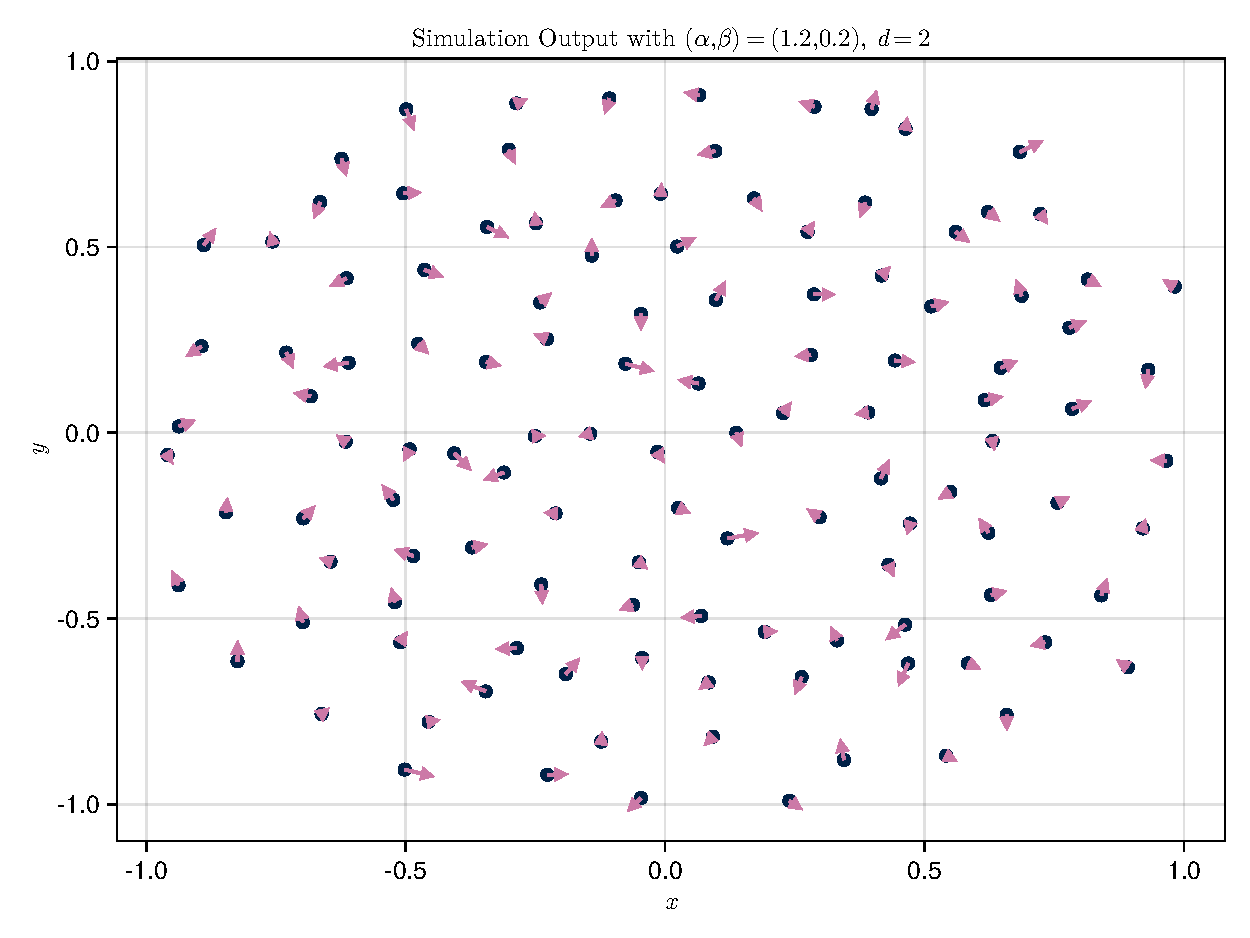
\includegraphics[width=0.72\linewidth]{results/known-2d/simulation-quiver.pdf}
  \caption[Quiver plot of 120 particles in 2D interacting through the attractive-repulsive potential]{Position and velocity of particles in the simulation at a point in time. Every particle, each of equal mass $m$, interacts with every other particle through the interaction potential $U_{ij} = K\left(\norm{\vec{x_i} - \vec{x_j}}\right)$ leading to $\mathcal{O}(N_p^2)$ interactions.}
  \label{fig:simulation-quiver}
\end{figure}

Because each particle interacts with every other particle, the number of interactions scales with $\mathcal{O}(N_p^2)$,
which can play a prohibitive role in terms of the computation time when increasing the number of particles $N_p \gg 1$.

Within the scope of this thesis, in order to understand the elaborate behaviour of such particle systems and also to verify results from theory and the spectral method, we provide an implementation of a simulator starting from a numerical time integrator in $\R^d$.
In addition to the \textit{headless} simulation software, exporting state and results for treatment by the analysis component, a \gls{gui} is provided to enable live insight into and interaction with the model, cf. \Cref{fig:gui-screenshot}.

\begin{figure}[H]
  \centering
  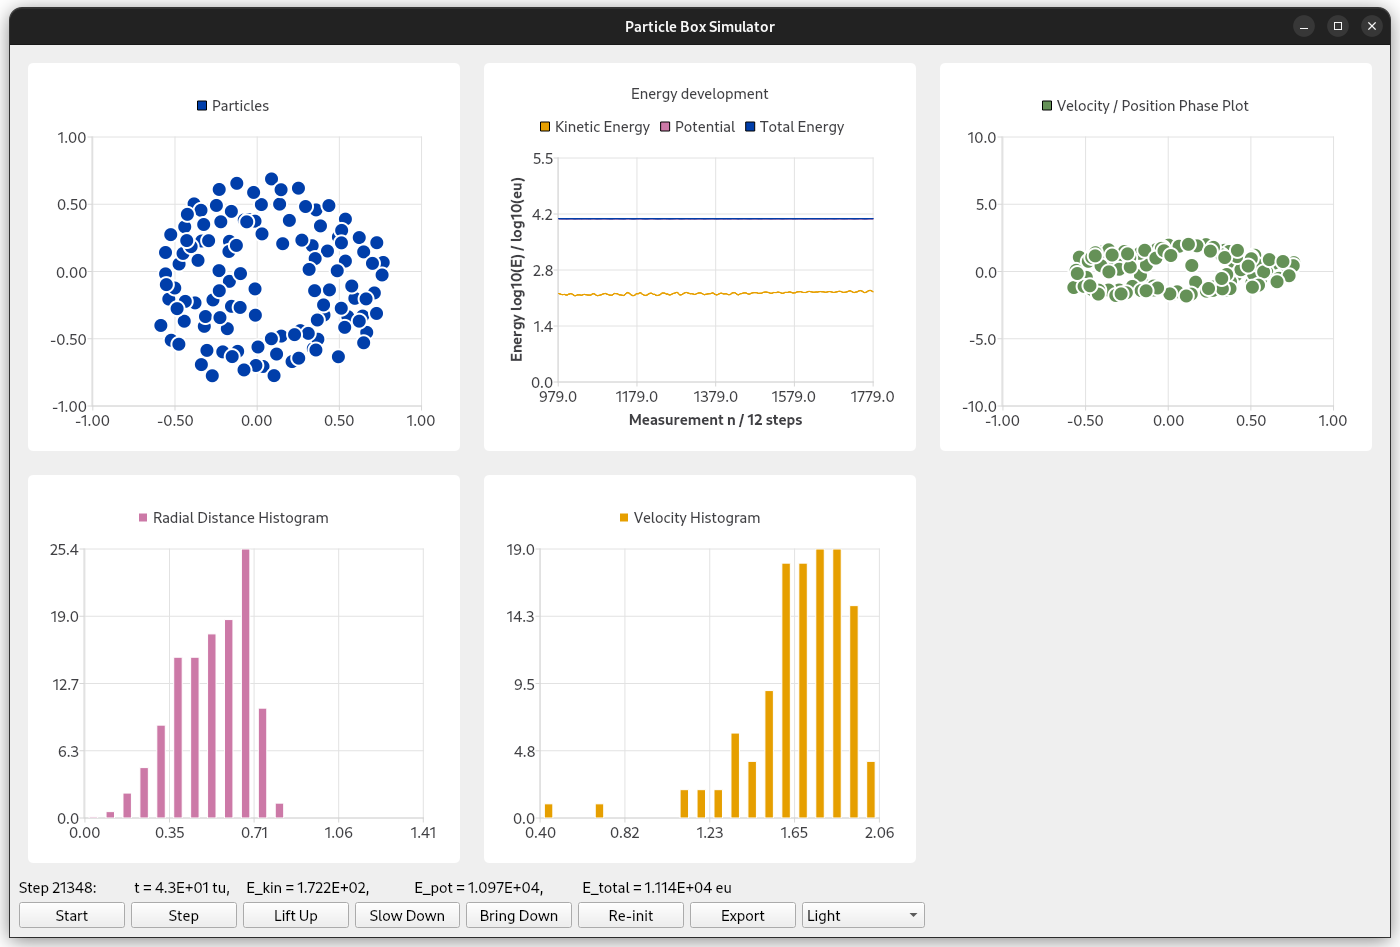
\includegraphics[width=\linewidth]{gui-screenshot.png}
  \caption[Graphical User Interface of the Simulator]{Screenshot of the \gls{gui} provided for the particle simulator. The top row shows the position of particles in their $[-1, 1]^d$ ($d = 2$ in this case) domain at a point $t$ in time, the energy development over time and the current position/velocity phase space plot. Below, there are position and velocity histogram updated live along with the simulation.}
  \label{fig:gui-screenshot}
\end{figure}

\begin{figure}[H]
  \centering
  \includegraphics[width=0.8\linewidth]{results/morse-3d/simulation-quiver-3d.pdf}
  \caption[Self-propelled particles in 3D interacting through $K_{C_a, l_a, C_r, l_r}(r)$.]{Self-propelled particles in a reflective box $[-1, 1]^3$ interacting via the Morse potential $K_{C_a, l_a, C_r, l_r}(r)$ in $d=3$ dimensions.}
  \label{fig:morse-3d-quiver}
\end{figure}

\section{Available Methods}
As a particular important problem in the physical sciences, there is an abundant number of simulation methods and solvers available for molecular dynamics problems.

Among them are simple forward integrators (e.g. $\vec{x_i}(t + \tau) \approx \vec{x_i}(t) + \tau \vec{v_i}(t)$ for $t > 0$ and timestep $\tau \in \R^+$), a generalisation of which are multistep methods.
Both essentially originate from expanding the position and velocity as Taylor series in time.
They work well in many general cases and error analysis is straightforward.

Named within the ``Top 10 Algorithms of the 20th Century'' \parencite{2000-top-algorithms}, the \gls{fmm} due to \cite{1987-multipole-method} uses a multipole expansion of the system's Green's function to cluster together interactions with far-away particles for physical interaction potentials such as the Coulomb- or gravitational potentials.
It does so by hierarchically clustering together particles based on position and treating interaction with far-away particles as a single interaction, therefore reducing the runtime from $\mathcal{O}(N_p^2)$ for each pair of particles down to $\mathcal{O}(N_p)$.
\gls{fmm} is among the few methods with rigorous results available on the error.
For long-range interactions however, as they are ubiquitous within this thesis (cf. the summary in \Cref{fig:comparing-potentials}), the \gls{fmm} is not applicable.

Another specialised method for the integration of Newton's equations of motion is leapfrog integration, our method of choice for the C++ implementation of the $N_p$-body simulator.

\subsection{Leapfrog Integration}
The Leapfrog algorithm is a more effective forward integration method due to its high resistance to numerical round-off error.
Except for minor changes in the way the velocity is updated, it is essentially the same as the velocity Verlet algorithm, a variant of Verlet integration with error on the order of $\mathcal{O}(\tau^4)$ with $\tau \in \R^+$ the timestep.

In particular, every particle $i$ at position $\vec{x_i} \in \R^d$ with velocity $\vec{v_i} \in \R^d$ is updated using
\begin{align*}
  \vec{x_i}(t+\tau)     & = \vec{x_i}(t)+\tau \cdot \vec{v_i}(t+\tau / 2),              & \quad\text{for}~ & t=0, \tau, \ldots\,,      \\
  \vec{v_i}(t+\tau / 2) & = \vec{v_i}(t-\tau/2) + \tau \cdot \vec{f}[\vec{x_i}(t), t],  & \quad\text{for}~ & t=\tau, 2 \tau, \ldots\,, \\
  \vec{v_i}(\tau / 2)   & = \vec{v_i}(0)+\frac{\tau}{2} \cdot \vec{f}[\vec{x_i}(0), 0], & \quad\text{for}~ & t=0\,,
\end{align*}
where $\vec{f_i}[\vec{x_i}(t), t] \in \R^d$ denotes the acceleration (sum of contributions of all forces divided by particle mass $m_i$).
Verlet integration methods are a common technique in molecular dynamics for the integration of Newton's equations of motion and implemented in many solvers.
Leapfrog integration can be improved to higher accuracy using Yoshida coefficients \parencite{1973-yoshida-coefficients}.
% TODO: vielleicht eine kleine Figure zur Visualisierung des Leap-Frogs
Our implementation can be found in \Cref{appendix:code-snippets}.

% TODO: where we note that $\nabla f(\norm{\vec{x}}) = \frac{\vec{x}}{\norm{\vec{x}}} f'(\norm{\vec{x}})$.

\section{Phase Space}
Each particle, at every point in time $t$, has a position and velocity value.
In $d=1$ dimension, one can visualise both of these quantities simultaneously in a phase space plot (cf. \Cref{fig:phase-space-plot}).
For $d > 1$ dimension, it is possible to either only visualise the first components $\{\vec{x_i}\}_1$ and $\{\vec{v_i}\}_1$ or to visualise the norm of the position (distance from the centre of mass) $r = \norm{\vec{x_i} - \vec{x}_{\text{centre}}}$ and velocity $\norm{\vec{v_i}}$.

\begin{figure}[H]
  \centering
  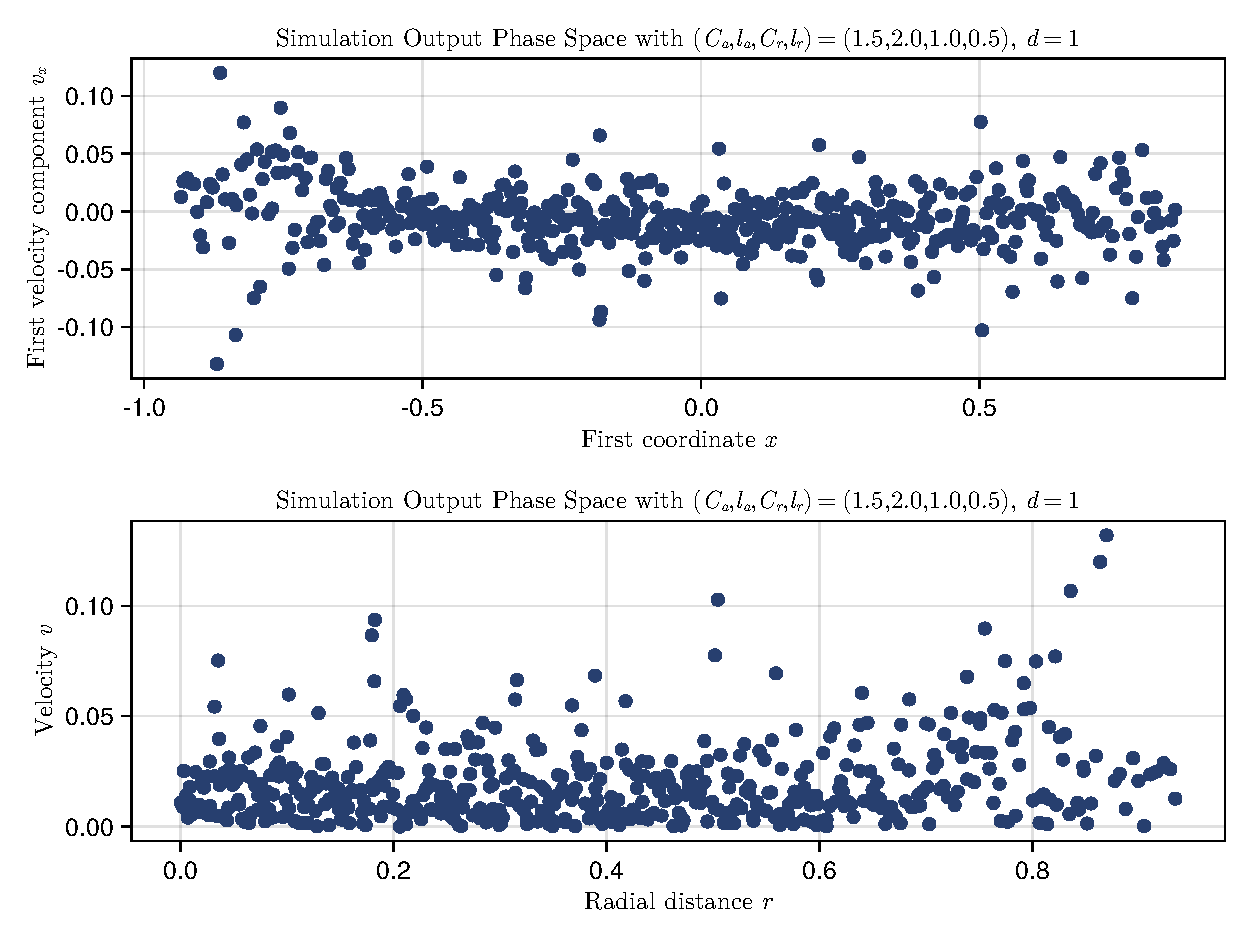
\includegraphics[width=0.8\linewidth]{results/morse/phase-space-plot.pdf}
  \caption[Phase Space Plots]{Position and velocity of $N_p = 500$ particles in a $d=1$ simulation visualised as phase space plots using the two different visualisation mechanisms. In the top plot, one can observe natural rotation around the origin $(0, 0)$ as positive velocity corresponds to movement to the right and negative velocity to leftwards movement. The colour indicates the $x$-coordinate of the particle, respectively (shown to visualise correspondence between the upper and the lower plot).}
  \label{fig:phase-space-plot}
\end{figure}

The behaviour of the phase space plot differs from potential to potential, most importantly one can observe multiple centers of rotation for the Morse potential in addition to the origin, whereas an attractive-repulsive potential builds up to an elliptical shape in the phase space plot.
% TODO: why is this? Local interactions?

\begin{figure}[H]
  \centering
  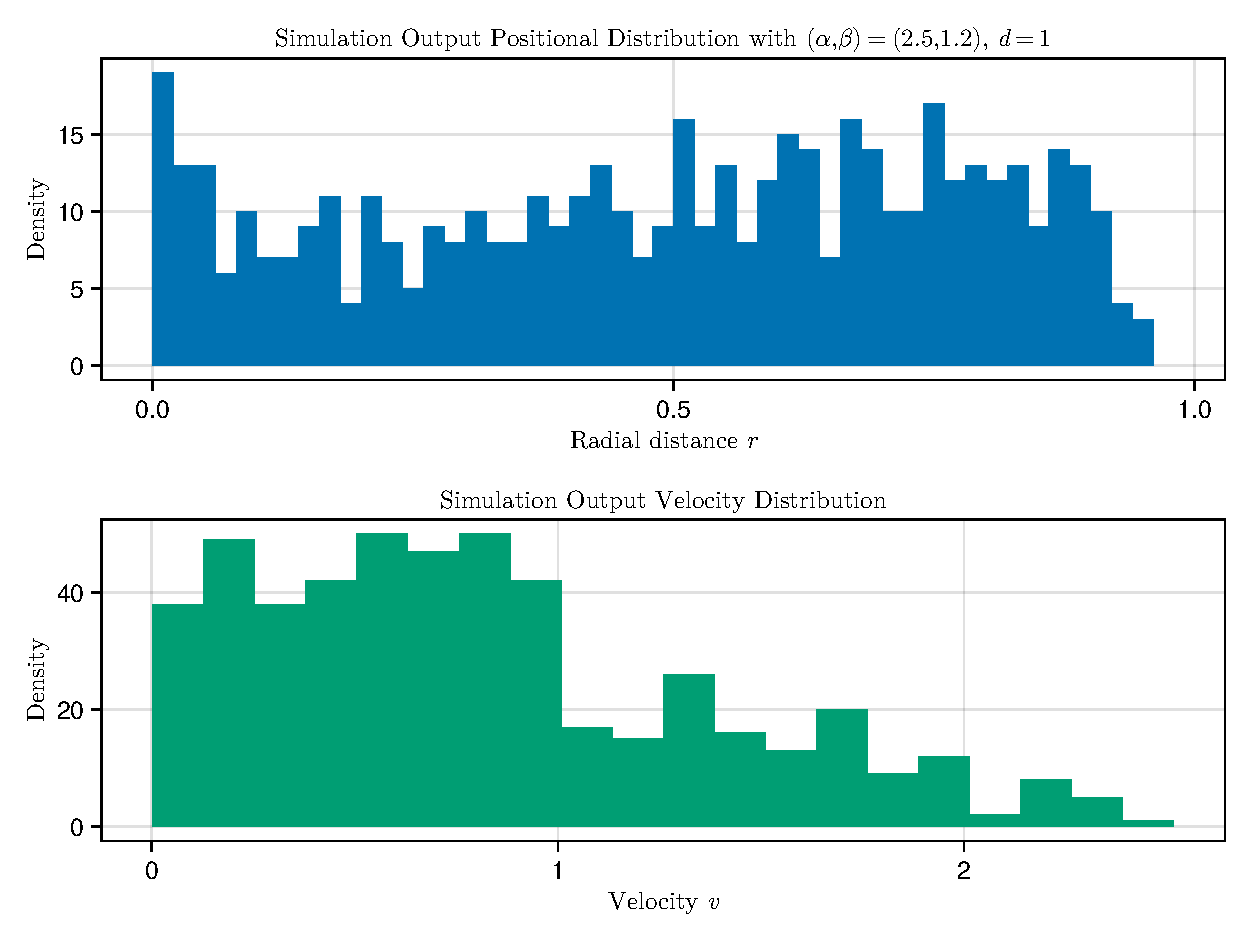
\includegraphics[width=0.8\linewidth]{results/attrep/simulation-histogram.pdf}
  \caption[Radial Distance and Velocity Histograms of attractive-repulsive Simulation Output in 1D]{Radial Distance ($r$) and Velocity ($v$) Histograms as obtained through a long-running simulation of $N_p = 500$ particles interacting through an attractive-repulsive potential $K_{\alpha, \beta}(r)$. The spectral method introduced in \Cref{chap:spectral-method} aims to solve for the particle density as a function of radial distance, hoping to predict the shape of the positional histogram.}
  \label{fig:simulation-histogram}
\end{figure}

In a physical setting with collision terms, the velocity distribution $f(\hat{v})$ would approach the shape of a Boltzmann distribution
$$f(\hat{v})={\bigg(\frac{m}{2\pi k_B T}\bigg)}^{\frac {3}{2}}\,4\pi \hat{v}^{2}\exp \left(-{\frac {m \hat{v}^{2}}{2k_B T}}\right)\,,$$
with $m$ the identical mass of each particle and velocity $\hat{v}$, $k_B$ the Boltzmann constant and $T \in \R^+$ is temperature, measured in Kelvin.
An exemplary velocity distribution is given in \Cref{fig:simulation-histogram}.

\section{Runtime Analysis}
\hierKoennteIhreWerbungStehen

\section{Further Experiments}
One can obtain interesting patterns using the absolute-value potential $K_{||}(r)$ as given in \Cref{eq:absvalue-potential} in $d=3$ dimensions, cf. \Cref{fig:gyroscope-quiver-3d,fig:fcc-quiver-3d}.
Because $K_{||}(r)$ is not continuously differentiable, the potential is not at all physical.
However, due to its linear penalty (instead of exponentials or power laws) it allows for a wider range of intriguing shapes of the collection of particles.

\begin{figure}[H]
  \centering
  \includegraphics[width=0.8\linewidth]{results/gyroscope-3d/simulation-quiver-3d.pdf}
  \caption{When running with $K(r) = |1-r|$ as an interaction potential and hence, $F(r) = -\nabla K(r) = -\sign(1-r)$, in $d=3$ dimensions a gyroscopic shape will form. The two outlying points are actually many particles above one another (high concentration of mass) and they form the axis of the rotating circle of particles.}
  \label{fig:gyroscope-quiver-3d}
\end{figure}

\begin{figure}[H]
  \centering
  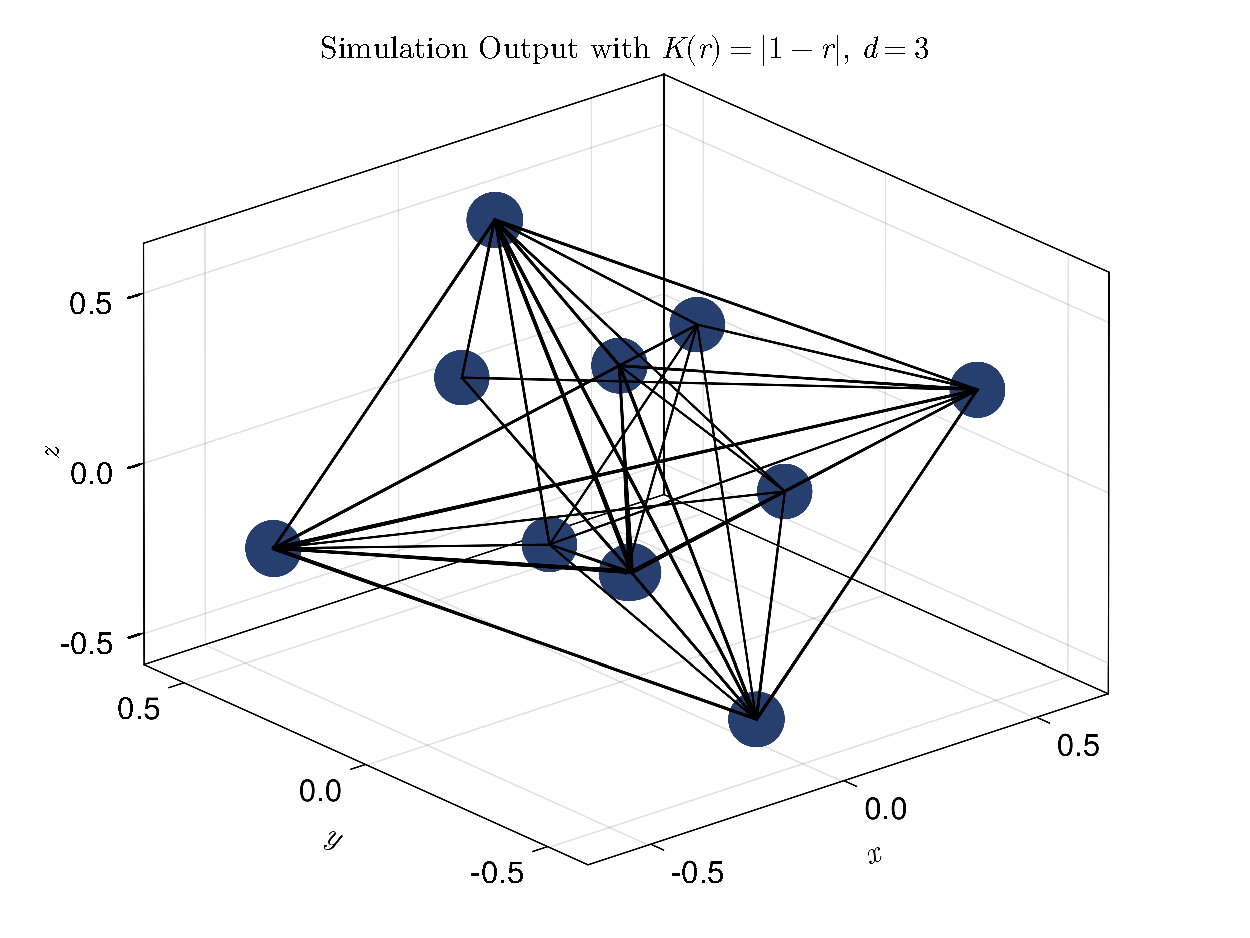
\includegraphics[width=0.8\linewidth]{results/gyroscope-3d/simulation-fcc-3d.pdf}
  \caption{When running an $N_p = 250$ particle simulation with $K(r) = |1-r|$ as an interaction potential in $d=3$ dimensions the particles will align into a stable ``optimal packing'' arrangement. In this case, they approximate a \gls{fcc} array of spheres, potentially providing a starting point for other algorithms.}
  \label{fig:fcc-quiver-3d}
\end{figure}

% TODO: add more details on the optimal packing? Maybe that this could be developed into an actual algorithm, etc.?
